\section{计算实现、CPU/GPU 对照与资源表现}
\label{chapter:10}

% block-id: 10.compute.heading
\hypertarget{10.compute.heading}{}
\subsection{CPU/GPU 数值对照与计算规模}

% block-id: 10.compute.p1
\hypertarget{10.compute.p1}{}
在相同模型、离散与积分设置下，5024 自由度的 CPU/GPU 部分电感矩阵相对差为 7.48×10⁻¹⁶，复电流相对差为 7.78×10⁻¹⁴；1264 自由度也达到 10⁻¹⁰ 对照门槛，见 图~\ref{fig:gpu_equivalence}。这些结果说明两种已实现算法在所比较矩阵与端口解上的数值一致性。性能比较还需要相同计时范围，本文保留各阶段时间及资源样本，物理结论采用前述模型验证结果。

% block-id: 10.compute.p2
\hypertarget{10.compute.p2}{}
图~\ref{fig:resource_memory} 给出可归属进程树的采样内存曲线，采样间隔内的短时峰值可能高于曲线所示值。更大规模中，9856 自由度保存了可恢复的部分电流等结果，其完整矩阵、公共电压或全场覆盖情况按数据清单逐项列出；20108 及以上规模提供资源需求和退出边界记录。它们用于评估进一步计算的成本，完整数值验证仍以具备相应检查数据的算例为依据。

% block-id: 10.workflow.heading
\hypertarget{10.workflow.heading}{}
\subsection{计算与文档构建}

% block-id: 10.workflow.p1
\hypertarget{10.workflow.p1}{}
研究计算入口读取模型输入和求解配置，输出运行记录及相应检查结果；文档构建入口读取已保存量值、图件与 LaTeX 主稿，生成 Markdown 阅读稿并编译预览 PDF。输入、源码及输出哈希共同定义一次构建，所用单图保留矢量曲线和字体信息，组图记录面板身份与布局参数。下列来源表用于从正文观测量追溯到具体文件及其验收记录。

% block-id: 10.figure.gpu_equivalence
\hypertarget{10.figure.gpu_equivalence}{}
\begin{figure}[!htbp]
\centering
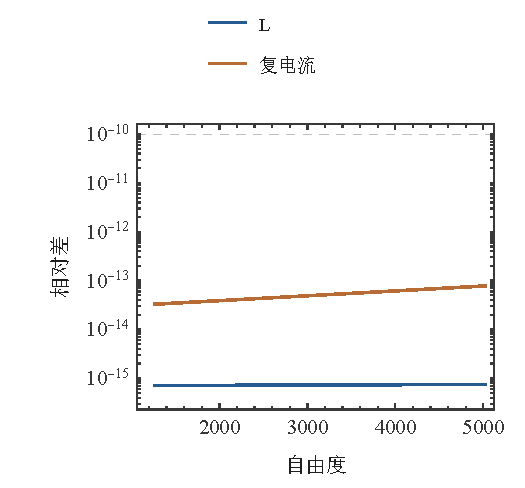
\includegraphics[width=\linewidth,height=.72\textheight,keepaspectratio]{../../assets/zh-CN/gpu_equivalence.pdf}
\caption{CPU/GPU 同模型数值对照。 矩阵与复电流相对差使用同一离散和积分设置。 相对差针对 1264 和 5024 自由度分别计算。水平参照为 10⁻¹⁰ 算法对照门槛。}
\label{fig:gpu_equivalence}
\end{figure}

% block-id: 10.figure.resource_memory
\hypertarget{10.figure.resource_memory}{}
\begin{figure}[!htbp]
\centering
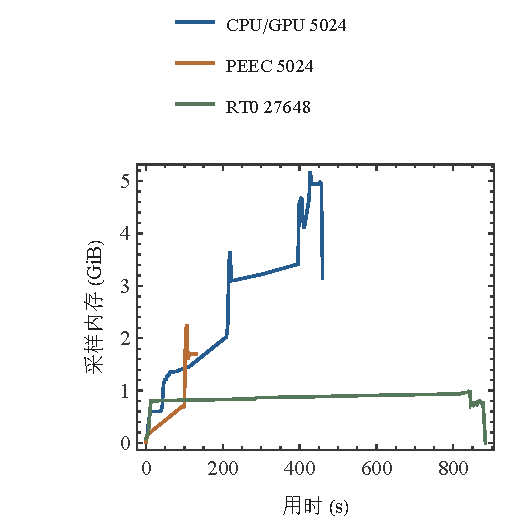
\includegraphics[width=\linewidth,height=.72\textheight,keepaspectratio]{../../assets/zh-CN/resource_memory.pdf}
\caption{可归属进程树资源曲线。 曲线使用归档的时间及内存样本。 时间以对应运行的起点归一化。内存为可归属进程树的采样工作集。}
\label{fig:resource_memory}
\end{figure}
